\documentclass[english]{MastersDoctoralThesis}\usepackage[]{graphicx}\usepackage[]{color}
%% maxwidth is the original width if it is less than linewidth
%% otherwise use linewidth (to make sure the graphics do not exceed the margin)
\makeatletter
\def\maxwidth{ %
  \ifdim\Gin@nat@width>\linewidth
    \linewidth
  \else
    \Gin@nat@width
  \fi
}
\makeatother

\definecolor{fgcolor}{rgb}{0.345, 0.345, 0.345}
\newcommand{\hlnum}[1]{\textcolor[rgb]{0.686,0.059,0.569}{#1}}%
\newcommand{\hlstr}[1]{\textcolor[rgb]{0.192,0.494,0.8}{#1}}%
\newcommand{\hlcom}[1]{\textcolor[rgb]{0.678,0.584,0.686}{\textit{#1}}}%
\newcommand{\hlopt}[1]{\textcolor[rgb]{0,0,0}{#1}}%
\newcommand{\hlstd}[1]{\textcolor[rgb]{0.345,0.345,0.345}{#1}}%
\newcommand{\hlkwa}[1]{\textcolor[rgb]{0.161,0.373,0.58}{\textbf{#1}}}%
\newcommand{\hlkwb}[1]{\textcolor[rgb]{0.69,0.353,0.396}{#1}}%
\newcommand{\hlkwc}[1]{\textcolor[rgb]{0.333,0.667,0.333}{#1}}%
\newcommand{\hlkwd}[1]{\textcolor[rgb]{0.737,0.353,0.396}{\textbf{#1}}}%
\let\hlipl\hlkwb

\usepackage{framed}
\makeatletter
\newenvironment{kframe}{%
 \def\at@end@of@kframe{}%
 \ifinner\ifhmode%
  \def\at@end@of@kframe{\end{minipage}}%
  \begin{minipage}{\columnwidth}%
 \fi\fi%
 \def\FrameCommand##1{\hskip\@totalleftmargin \hskip-\fboxsep
 \colorbox{shadecolor}{##1}\hskip-\fboxsep
     % There is no \\@totalrightmargin, so:
     \hskip-\linewidth \hskip-\@totalleftmargin \hskip\columnwidth}%
 \MakeFramed {\advance\hsize-\width
   \@totalleftmargin\z@ \linewidth\hsize
   \@setminipage}}%
 {\par\unskip\endMakeFramed%
 \at@end@of@kframe}
\makeatother

\definecolor{shadecolor}{rgb}{.97, .97, .97}
\definecolor{messagecolor}{rgb}{0, 0, 0}
\definecolor{warningcolor}{rgb}{1, 0, 1}
\definecolor{errorcolor}{rgb}{1, 0, 0}
\newenvironment{knitrout}{}{} % an empty environment to be redefined in TeX

\usepackage{alltt}

\usepackage{amsmath}
\usepackage{amsfonts}

\usepackage[utf8]{inputenc}
\usepackage[T1]{fontenc}

\usepackage{mathpazo} % Use the Palatino font by default

\usepackage[backend=bibtex,style=authoryear,natbib=true]{biblatex}

% plan to remove these
\newcommand{\bB}{\mathbf{B}}
\newcommand{\bbeta}{\boldsymbol\beta}
\newcommand{\bbetahat}{\boldsymbol{\hat\beta}}
\newcommand{\bY}{\boldsymbol Y}
\newcommand{\bX}{\boldsymbol X}
\newcommand{\bx}{\boldsymbol x}
\newcommand{\bz}{\boldsymbol z}
\newcommand{\bbX}{\textbf{X}}



%% new symbol list, better structured

\newcommand{\mat}[1]{\mathbf{#1}}
\renewcommand{\vec}[1]{\boldsymbol{#1}}
\newcommand{\tvec}[1]{\left[#1\right]^\top}
\newcommand{\collect}[1]{\left\{#1\right\}}

\newcommand{\Vtime}{t}
\newcommand{\Vtdiff}{\delta}

\newcommand{\Vobs}{\boldsymbol{y}}
\newcommand{\VobsMat}{\mat Y}
\newcommand{\Vlat}{\phi}
\newcommand{\Vlon}{\lambda}
\newcommand{\Varr}{A}
\newcommand{\Vdep}{D}
\newcommand{\Vdwell}{\tilde\Vdep}

\newcommand{\Vstate}{\bx}
\newcommand{\Vdist}{x}
\newcommand{\Vspeed}{\dot x}
\newcommand{\Vaccel}{\ddot x}
\newcommand{\Vtt}{B}
\newcommand{\Vttobs}{b}
\newcommand{\Vtterr}{e}
\newcommand{\Np}{N}
\newcommand{\Pwt}[1][i]{w^{(#1)}}
\newcommand{\Vtrans}{f}
\newcommand{\Vmeas}{h}
\newcommand{\Vprojf}{g}
\newcommand{\Vproj}[2]{g\left(#1\,|\,#2\right)}
\newcommand{\Viproj}[2]{g^{-1}\left(#1\,|\,#2\right)}
\newcommand{\Vnoise}{\sigma^2}
\newcommand{\GPSerrSD}{\varepsilon}
\newcommand{\GPSerr}{\GPSerrSD^2}
\newcommand{\TUerrSD}{\xi}
\newcommand{\TUerr}{\TUerrSD^2}
\newcommand{\Ppos}{\vec{\tilde Y}}

\newcommand{\Neff}{N_\text{eff}}
\newcommand{\Nthres}{N_\text{thres}}

\newcommand{\Vsegstart}{T}
\newcommand{\Vsegend}{T'}

\newcommand{\vi}[1][i]{^{(#1)}}

\newcommand{\Nstop}{M}
\newcommand{\Nseg}{L}
\newcommand{\Tstopd}{\mathcal{S}}
\newcommand{\Tsegd}{\mathcal{D}}
\newcommand{\Tseglen}{\mathcal{L}}
\newcommand{\Prstop}{\pi}
\newcommand{\mindwell}{\gamma}
\newcommand{\dwell}{\tau}
\newcommand{\dwellvar}{\omega^2}
\newcommand{\Istop}{p}
\newcommand{\pdwell}{d}
\newcommand{\pserve}{\tilde d}
\newcommand{\Print}{\rho}
\newcommand{\intwait}{\nu}
\newcommand{\Iint}{r}
\newcommand{\pwait}{w}
\newcommand{\pcwait}{\tilde w}

\newcommand{\NWtdiff}{\Delta}
\newcommand{\NWstate}{\beta}
\newcommand{\NWstatevar}{\mat{P}}
\newcommand{\NWvar}{\mat{\boldsymbol{\psi}}}
\newcommand{\Rstate}{b}
\newcommand{\Rvar}{v}
\newcommand{\NWnoise}{q}
\newcommand{\NWerr}{\Vtterr}
\newcommand{\NWtransfun}{F}
\newcommand{\NWtrans}{\mat{\NWtransfun}}
\newcommand{\NWmeas}{\mat{H}}
\newcommand{\NWobss}{Z}
\newcommand{\NWobs}{\Vttobs}
\newcommand{\NWErr}{E}
\newcommand{\NWinfmat}{\mat{U}}
\newcommand{\NWinfvec}{\boldsymbol{u}}
\newcommand{\NWobsinfmat}{\mat{I}}
\newcommand{\NWobsinfvec}{\boldsymbol{i}}
\newcommand{\NWctrl}{\xi}
\newcommand{\NWctrlvec}{\vec\NWctrl}
\newcommand{\NWmaxtt}{\mu}
\newcommand{\MaxSpeed}{\mathbb{V}}

\newcommand{\NWhistmean}[2]{\beta_{#1}\left(#2\right)}
\newcommand{\NWhistvar}[2]{\psi_{#1}\left(#2\right)}
\newcommand{\NWmeantt}{\theta}
\newcommand{\NWvartt}{\omega^2}

\newcommand{\ellc}{\ell,c}

\newcommand{\Linkt}{\eta}
\newcommand{\Linktt}{\boldsymbol{\Linkt}}
\newcommand{\Nodedwell}{\kappa}
\newcommand{\Tarr}{\alpha}
\newcommand{\TTarr}{\boldsymbol{\Tarr}}
\newcommand{\Tdwell}{\Delta}
\newcommand{\TTdwell}{\boldsymbol{\Tdwell}}
\newcommand{\TripTime}{{t_r}}

\newcommand{\RouteNWstate}{\Theta}
\newcommand{\RouteNWstateseg}{\theta}
\newcommand{\RouteNWstatesegvar}{P}
\newcommand{\RouteNWstatecor}{\rho}

\newcommand{\Tripr}{\mathcal{T}}
\newcommand{\Tript}{t}
\newcommand{\TripStop}{s}
\newcommand{\TripDep}{d}
\newcommand{\TripSeg}{r}
\newcommand{\SegProg}{\zeta}

\newcommand{\FM}{\mathcal{F}}

\newcommand{\RouteSegs}{\mathcal{R}}
\newcommand{\ShapePath}{\mathcal{P}}

\newcommand{\dist}[1]{d\left(#1\right)}
\newcommand{\distThreshold}{D_\text{thres}}

% distributions
\newcommand{\Normal}[2]{\mathcal{N}\left(#1,\, #2\right)}
\newcommand{\TNormal}[4]{\mathcal{N}_T\left(#1,\, #2,\, #3,\, #4\right)}
\newcommand{\LogNormal}[2]{\log\text{-}\mathcal{N}\left(#1,\, #2\right)}
\newcommand{\Bern}[1]{\mathrm{Bernoulli}\left(#1\right)}
\newcommand{\Exp}[1]{\mathcal{E}\left(#1\right)}
\newcommand{\GammaD}[2]{\mathcal{G}\left(#1,\, #2\right)}
\newcommand{\Uniform}[2]{\mathcal{U}\left(#1,\, #2\right)}

% other stuff
\newcommand{\E}[1]{\mathbb{E}\left[#1\right]}
\newcommand{\Var}[1]{\mathrm{Var}\left[#1\right]}
\newcommand{\Cov}[2]{\mathrm{Cov}\left[#1,\,#2\right]}
\newcommand{\dirac}{\dot\delta}
\newcommand{\DiracMeasure}[2]{\dirac_{#1}\left(#2\right)}
\renewcommand{\Pr}[1]{\mathbb{P}\left(#1\right)}

\newcommand{\cond}{\,\big|\,}

\newcommand{\Pcatch}{\mathbb{P}_\text{catch}}
\newcommand{\Ptransfer}{\mathbb{P}_\text{transfer}}
\newcommand{\Ewait}{\mathbb{E}_\text{wait}}
\newcommand{\Ecatch}{\mathbb{E}_\text{catch}}
\newcommand{\Emiss}{\mathbb{E}_\text{miss}}

\newcommand{\th}{^\text{th}}
\newcommand{\dx}{\,\mathrm{d}x}

\let\oldemptyset\emptyset
\let\emptyset\varnothing

\begin{symbols}{lll} % Include a list of Symbols (a three column table)

% time symbols
$\Vtime_k$      & time of the $k^{\text{th}}$ observation & Unix timestamp \\
$\Vtdiff_k$     & time since the last observation & seconds \\
\addlinespace

% vehicle observation symbols
$\Vobs_k$     & vehicle observation (at time $\Vtime_k$) & \\
$\Vlat_k$     & vehicle latitude & degrees \\
$\Vlon_k$     & vehicle longitude & degrees \\
$\Varr_m$     & vehicle arrival time at stop $m$ & Unix timestamp \\
$\Vdep_m$     & vehicle departure time from stop $m$ & Unix timestamp \\
$\Vdwell_m$   & vehicle dwell time at stop $m$ & seconds \\
\addlinespace

% vehicle state symbols
$\Vstate_k$   & vehicle state (at time $\Vtime_k$) & \\
$\Vdist_k$    & vehicle distance into trip & m \\
$\Vdist_k$    & vehicle speed & m/s \\
$\Vtt_\ell$   & vehicle travel time along segment $\ell$ & seconds \\
$\Np$         & number of particles per vehicle & \\
$\Pwt_k$      & weight of particle $i$ given observation at time $\Vtime_k$ & \\
$\Vtrans$     & vehicle transition function & \\
$\Vmeas$      & vehicle measurement function & \\
$\Vprojf$     & equirectangular projection function & \\
$\Vnoise$     & vehicle model system noise & m/s \\
$\GPSerr$     & GPS error & meters \\
$\TUerr$      & Trip update arrival/departure error & seconds \\
$\Ppos\vi_k$  & Particle GPS position & \\
\addlinespace

% trip symbols
$\Nstop_r$      & number of stops in trip $r$ & \\
$\Nseg_r$       & number of segments in trip $r$ & \\
$\Tstopd_m$     & distance into trip of stop $m$ & meters \\
$\Tsegd_\ell$   & distance into trip of start of segment $m$ & meters \\
$\Tseglen_\ell$ & length of segment $m$ & meters \\
$\Prstop_m$     & probability of stopping at stop $m$ & \\
$\mindwell$     & minimum dwell time & seconds \\
$\dwell_m$      & mean dwell time at stop $m$ & seconds \\
$\dwellvar_m$   & variance of dwell time at stop $m$ & seconds \\
$\Istop_m$      & indicator that vehicle stopped at stop $m$ & \\
$\Print_\ell$   & probability of stopping at intersection $\ell$ & \\
$\intwait_\ell$ & mean wait time at intersection $\ell$ & seconds \\
$\Iint_m$       & indicator that vehicle stopped at intersection $\ell$ & \\
\addlinespace

% network symbols
$\NWstate_c$        & road network state (travel time, at time $t_c$)   & seconds \\
$\NWvar_c$          & road network state (travel time) variance & seconds \\
% $\Rstate_{\ell c}$  & travel time along road segment $\ell$ & seconds \\
% $\Rvar_{\ell c}$    & travel time variance along road segment $\ell$ & seconds \\
$\NWnoise_c$        & road network system noise matrix & seconds \\
%$\NWmeas_c$         & road network measurement error matrix & seconds \\
$\NWobs_c$          & road network observation vector & seconds \\
$\NWinfmat_c$       & road network information matrix & \\
$\NWinfvec_c$       & road network information vector & \\
\addlinespace

$\NWhistmean{\ell}{t_c}$ & historical mean travel time (along segment $\ell$ at time $t_c$) & seconds \\
$\NWhistvar{\ell}{t_c}$  & historical variance of travel time & seconds \\

% ETA symbols
$\Linktt_r$      & vector of inter-stop (link) travel times for trip $r$ & seconds \\
$\TTarr_r$       & vector of arrival times for trip $r$ & seconds \\
$\TTdwell_r$      & vector of node dwell times for trip $r$ & seconds \\
$\TripTime_r$    & the time trip $r$ was last updated \\

\end{symbols}



\title{Tom's awesome thesis on buses}
\author{Tom Elliott}
\date{2019}
\IfFileExists{upquote.sty}{\usepackage{upquote}}{}
\begin{document}

\maketitle

\tableofcontents
\tabularnewline

\frontmatter

\chapter*{Abstract}

This is the abstract.

\mainmatter
% Main chapters



\chapter{Introduction}

This is the intro. Literature review, the problem,
and the goals of this work (i.e., to make better predictions
that don't rely on the timetable).

\part{Real-time bus models}



\chapter{Literature review}

This is a ``review'' of what's been happening in the field of
bus arrival-time prediction and modeling.
From its routes in Kalman filtering,
through fancy ANN and SVM models,
to computer intensive particle filter models
(not for real-time applications).

What's missing: focus on improved arrival-time prediction,
rather than an OR approach.



\chapter{GTFS data and route segmentation}

Talk about the data itself: where it comes from,
the important aspects we care about
(trips/routes, shapes, stops, and stop times).


\section{Real-time data}

What's involved, frequency, and some of the
quirks (at least in our Auckland Transport example).


\section{Segmentation of routes}

This is cool --- by segmenting routes
(at intersections) we remove dependency of
speed/travel time on \emph{route} and instead
relate it to the physical road the vehicle is traveling along.



\chapter{Transit vehicle model}
\label{cha:vehiclemodel}

This chapter should be about the model itself,
including traffic lights, dwell times, speed, etc.
It's a recursive Bayesian model,
which means the state at time $k$ is a function
of the state at time $k-1$.

\section{Particle filter}

About how it's actually implemented using a particle filter,
and the reasons why we chose that.


\part{Transit network}



\chapter{Constructing a GTFS network}

Here we give a detailed overview of what exactly the
transit network is
(in the previous chapter, we only alluded to it,
and assumed segments where known).

The basic idea of splitting shapes at intersections,
which we get manually, or could potentially
obtain using shape-processing methods.

Some of the slight issues, e.g., missing intersections.



\chapter{Real-time network model}

%The modified Kalman filter approach to modeling
%travel times as vehicles travel along each
%road segment.


The \emph{network state} is denoted by $\bbeta$,
a vector of length $L$, the number of segments in the network.
Each $\beta_\ell$ represents the \emph{mean travel time} of buses
in segment $\ell$.
To denote time, we add a $c$ subscript to the state, $\bbeta_c$
and $\beta_{c\ell}$.

The \emph{state estimate} will be denoted as $\bbetahat$.

\section{Predict step}

The first step in the EKF process is to predict the state at time $c$.
Here we wish to estimate $\bbetahat_{c|c-1}$, the network state at time $c$,
given the posterior state estimate at time $c-1$.

\subsection{Transition function}

Based on an extended Kalman filter,
the transition function $f$ defines the state at time $c$
as a deterministic function of the state at time $c-1$
and system noise, $u_c \sim \mathcal{N}(0, Q)$.
That is,
\begin{equation}
    \label{eq:kf_transition_basic}
    \bbetahat_{c|c-1} = f(\bbetahat_{c-1|c-1}, u_c).
\end{equation}

The next step is to define $f$ so that it meets the criteria for
the EKF (it must be differentiable), and has the properties we desire:
that the state will regress to the prior in the absense of any observations.

To bring the state towards the prior mean travel time for segment $\ell$,
$\nu_\ell$, we define the transition function for a single second, $f$, as
\begin{equation}
    \label{eq:kf_transition_def}
    f(\beta_{\ell,c}, \nu_\ell, \lambda) = \beta_{\ell,c-1} + \lambda (\nu_\ell - \beta_{\ell,c-1})
\end{equation}
where $\lambda \in (0,1)$ is a tuning parameter that determines the rate at which
the state converges.
We can easily calculate the derivative of $f$, too, which is a requirement for the EKF.
\begin{equation}
    \label{eq:kf_transition_fderiv}
    f'(\beta_{\ell,c}, \nu_\ell, \lambda) = 1 - \lambda
\end{equation}

Next we need to be able to define the a transition for $\Delta$ seconds,
which by recursion of \ref{eq:kf_transition_def} is
\begin{equation}
    \label{eq:kf_transition_n}
    f_n(\beta_{\ell,c-1}, \nu_\ell, \lambda) =
    (f^1 \circ \cdots \circ f^n)(\beta_{\ell,c=1}, \nu_\ell, \lambda), \quad\text{where } f^j\equiv f\quad \forall j.
\end{equation}

The derivative of \ref{eq:kf_transition_n} is obtained used the chain rule,
$f(g(x))' = f'(g(x)) g'(x)$.
We will use $f(\beta) \equiv f(\beta_{\ell,c-1},\nu_\ell,\lambda)$ to simplify notation
(the other parameters are constant).
\begin{align}
    \label{eq:kf_transition_F}
    \F_n = f'_n(\beta) &=
    f'\left((f^1\circ\cdots\circ f^{n-1})(\beta)\right)(f^1\circ\cdots\circ f^{n-1})'(\beta) \nonumber \\
    &= f'\left(f_{n-1}(\beta)\right) \F_{n-1} \nonumber \\
    &= f'\left(f_{n-1}(\beta)\right) f'\left(f_{n-2}(\beta)\right) \cdots f'\left(f_1(\beta)\right) f'(\beta) \nonumber \\
    &= f'(\beta) \prod_{i=1}^{n-1} f'\left(f_i(\beta)\right) \nonumber \\
\intertext{Substituting \ref{eq:kf_transition_fderiv}, we get}
    \F_n &= (1-\lambda) \prod_{i=1}^{n-1}(1-\lambda) = (1-\lambda)^n
\end{align}


Next we need to ensure the entire state, and not just the mean,
converges to the prior,
i.e., the state variance $P_{\ell,c}$ converges to the prior variance, $\xi_{\ell} = \xi_\ell$.

The system noise, $Q$, is used to predict the state variance,
\begin{equation}
    \label{eq:kf_transition_predvar}
    P_{\ell,c|c-1} = F_n^2 P_{\ell,c-1|c-1} + L_c Q
\end{equation}
At convergence, we want $P_{\ell,c|c-1} = P_{\ell,c-1|c-1} = \xi_\ell$, and
$L_{c-1} = \left.\frac{\partial f_n}{\partial u}\right|_{\hat\beta_{\ell,c|c-1}} = 1$.
Substituting into \ref{eq:kf_transition_predvar} and solving for $Q$:
\begin{align}
    \label{eq:kf_transition_Q}
    \xi_\ell &= F^2_n\xi_\ell + Q \nonumber \\
    &= (1-\lambda)^{2n}\xi_\ell + Q \nonumber \\
    Q &= \xi_\ell(1 - (1 - \lambda)^{2n})
\end{align}

Now that the state will converge to the prior,
the last thing we have to do is determine how fast it does so.
This is controlled by $\lambda$;
however, we want the rate of convergence to be slow
after an observation, and speed up the longer we go without seeing any buses.
That is, we want to use a ratio of $P_\ell$ and $\xi_\ell$,
\begin{equation}
    \label{eq:kf_transition_lambda}
    \lambda = \phi \frac{P_{\ell,c-1|c-1}}{P_{\ell,c-1|c-1} + \xi_\ell}
\end{equation}
where $\phi$ is a tuning parameter.



\section{Update step}

Having predicted the state at time $t_c$,
we can now update our estimate based on the observed data,
$\bB_c$, which consists of the combined travel times
of all $K_m$ vehicles completing travel along the segment
during the current iteration.
For each vehicle, we can obtain the mean and uncertainty
of travel time from the particle filter,
$b_{v,\ell}$ and $e_{v\ell}$, respectively.
These can then be combined to obtain a single observation for the EKF,
along with an estimate to use as measurement error:
\begin{align}
    \label{eq:kf_update_B}
    B_{\ell,c} &= \frac{1}{K_m} \sum_{v=1}^{K_m} b_{v,\ell} \\
    \label{eq:kf_update_E}
    \hat E_{\ell,c} &= \frac{1}{K_m} \sum_{v=1}^{K_m}
        \left(b_{v,\ell}^2 + e_{v,\ell}^2\right) - B_{\ell,c}
\end{align}

Now the EKF proceeds as normal,
so we only need to define the measurement function, $h$,
which defines how the true state $\nu_{\ell,c}$ is related to the observed state, $\beta_{\ell,c}$.
\begin{equation}
    \label{eq:kf_measure}
    \nu_{\ell,c} = h(\beta_{\ell,c}, e_{\ell,c}) = \beta_{\ell,c} + e_{\ell,c},
    \quad e_{\ell,c}\sim \mathcal{N}(0, \hat E_{\ell,c})
\end{equation}

Before we can complete the update step of the EKF algorithm, we need to calculate two more derivatives:
\begin{align}
    \label{eq:kf_update_H}
    H_c = \left.\frac{\partial h}{\partial \nu}\right|_{\hat\beta_{\ell,c|c-1}} &= 1 \\
    M_c = \left.\frac{\partial h}{\partial e}\right|_{\hat\beta_{\ell,c|c-1}} &= 1
\end{align}
As we are using additive effects, these are both 1;
however, setting it out this way allows us to switch to using multiplicative
noise terms in future.

Now we can update the state estimates
\begin{align}
    \label{eq:kf_update_resid}
    \tilde y_c &= B_{\ell,c} - h(\hat\beta_{\ell,c|c-1}) \\
    \label{eq:kf_update_Sk}
    S_c &= H^T P_{\ell,c|c-1} H + M^T \hat E_{\ell,c} M \\
    \label{eq:kf_update_gain}
    K_c &= P_{\ell,c|c-1} H_c S_c^{-1} \\
    \label{eq:kf_update_statemean}
    \hat\beta_{\ell,c|c} &= \hat\beta_{\ell,c|c-1} + K_c\tilde y_c \\
    \label{eq:kf_update_statevar}
    P_{\ell,c|c} &= (I - K_c H) P_{\ell,c|c-1}
\end{align}

And here's what that looks like when implemented for a single segment.
\begin{knitrout}
\definecolor{shadecolor}{rgb}{0.969, 0.969, 0.969}\color{fgcolor}\begin{kframe}
\begin{alltt}
\hlstd{x} \hlkwb{<-} \hlnum{1}\hlopt{:}\hlnum{10}
\hlkwd{plot}\hlstd{(x)}
\end{alltt}
\end{kframe}
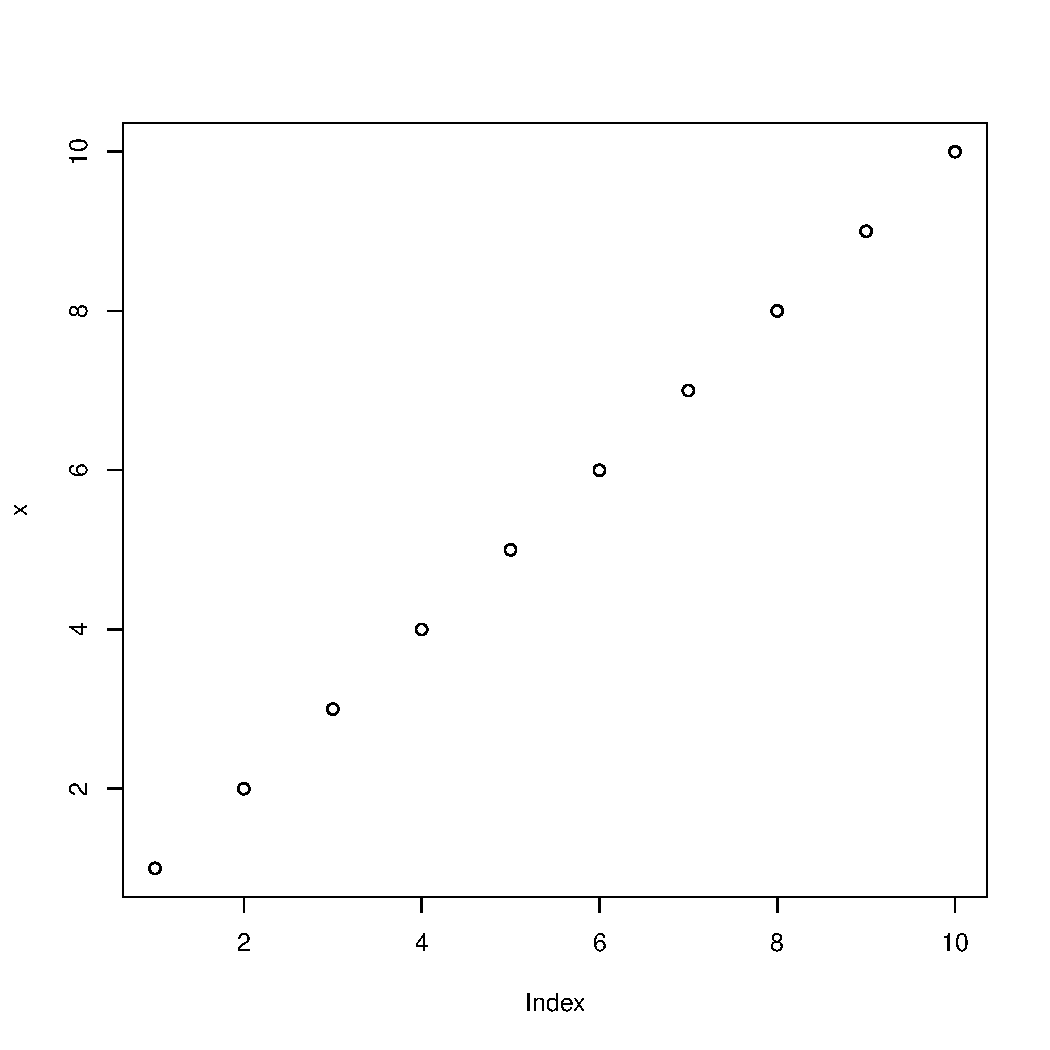
\includegraphics[width=\maxwidth]{figure/kf_eg-1} 

\end{knitrout}




\chapter{Historical data based priors}
\label{cha:historymodel}

How we use Bayesian heirarchical models to
estimate the typical speed along roads in the
network, based on historical data.


\appendix
% knit_child('endmatter/appendix/app1.Rnw')



\end{document}
